%==============================================================================
\chapter{Grundlagern der Kraftstoffsysteme von Fluggasturbinen}\label{chap:grundlagen}

Im folgenden Kapitel werden die Grundlagen von Kraftstoffsystemen für kerosinbetriebene und wasserstoffbetriebene Fluggasturbinen erläutert.

\section{Kerosin-Kraftstoffsysteme}

Die Hauptfunktion des Kerosin-Kraftstoffsystems besteht darin, den erforderlichen Kraftstoffmassenstrom zur Brennkammer zu fördern und vorzukonditionieren \cite{Jackson.2015}. Insbesondere muss der Kraftstoff mit einem Überdruck zur Brennkammer gepumpt werden, um eine zuverlässige Zerstäubung durch die Einspritzdüsen der Brennkammer sicherzustellen. 

Die Regelung von Kraftstoffdruck und  -massenstrom erfolgt durch eine Kombination aus Kraftstoffpumpen und der Kraftstoffregeleinheit (engl.: Fuel Metering Unit, FMU) \cite{Braunling.2015}. Zur Vorkonditionierung des Kraftstoffs gehört auch die Erwärmung. Während des Reiseflugs in großer Höhe kühlt der Kraftstoff in den Tanks durch die kalte Umgebungsluft stark ab. Da eine zu niedrige Kraftstofftemperatur das Risiko von Verstopfungen durch im Kraftstoff gelöste Eiskristalle birgt, wird der Kraftstoff in mehreren Wärmeübertragern erwärmt \cite{Doman.2015}. Durch die Nutzung der Abwärme anderer Triebwerkssysteme zur Kraftstofferwärmung kann gleichzeitig die Sekundärfunktion der Triebwerkskühlung erfüllt werden \cite{Braunling.2015, Jackson.2015}. Auch eine erhöhte Kraftstofftemperatur kann zu Problemen in Form von Dampfblasenbildung führen. Es ist daher notwendig die Kraftstoff- und Öltemperaturen über ein Wärmemanagementsystem zu regeln \cite{Braunling.2015}. 

In diesem Kapitel werden zunächst die Eigenschaften der Komponenten der Kerosin-Kraftstoffsysteme beschrieben. Anschließend wird eine mögliche Anordnung dieser Komponenten am Beispiel des CFM International CFM56-5B Triebwerks vorgestellt – einem etablierten Triebwerk für Schmalrumpfverkehrsflugzeuge.



\subsection{Kraftstoffpumpen und Regelung}

Die Triebwerke moderner Verkehrsflugzeuge werden im regulären Betrieb mithilfe elektrisch betriebener Boosterpumpen mit Kraftstoff aus den Flügel- und Rumpftanks versorgt. Diese Boosterpumpen stellen eine Druckmarge zum Sättigungsdampfdruck des Kraftstoffs sicher, um Kavitation in den Kraftstoffpumpen der Triebwerke zu vermeiden. In Kerosin-Kraftstoffsystemen ist die Druckerhöhung in der Regel auf zwei Kraftstoffpumpen aufgeteilt, die sich ein Gehäuse teilen und beide über den Hilfsgeräteträger von der Hochdruckwelle angetrieben werden. \cite{Braunling.2015}

Die Niederdruck-Kraftstoffpumpe (engl.: Low-Pressure Fuel Pump, LPFP) ist üblicherweise als Kreiselpumpe ausgeführt. Ihre Aufgabe besteht darin, die Druckverluste im Niederdrucksystem zu kompensieren, sodass auch im Einlauf der Hochdruck-Kraftstoffpumpe (engl.: High-Pressure Fuel Pump, HPFP) eine  Druckmarge zum Sättigungsdampfdruck des Kraftstoffs sichergestellt ist. Als bevorzugte Bauweise für die Hochdruckpumpe hat sich die Verdrängerpumpe, insbesondere in Form einer Zahnradpumpe, etabliert, da sie  die erforderlichen Austrittsdrücke in einer einzelnen Stufe erreicht. \cite{Braunling.2015}

Da eine Verdrängerpumpe unabhängig vom Kraftstoffbedarf bei gegebener Drehzahl ein konstantes Volumen fördert, ist eine Regelung des Kraftstoffmassenstroms erforderlich. Diese Regelung erfolgt durch eine Kombination aus Sensoren und Ventilen innerhalb der Kraftstoffregeleinheit. Der überschüssige Kraftstoff (engl.: spill-over), der über die Ventile abgeführt wird, wird teilweise in das Niederdrucksystem und teilweise in die Kraftstofftanks zurückgeführt. \cite{Braunling.2015}

\subsection{Wärmeübertrager}

In konventionellen Kraftstoffsystemen kommen üblicherweise zwei Wärmeübertrager (engl.: Fuel Oil Heat Exchanger, FOHE) zum Einsatz. Einer davon kühlt das Ölsystem des Stromgenerators (engl.: Integrated Drive Generator, IDG), während der andere das Hauptölsystem und damit indirekt die Lager und das Getriebe des Triebwerks kühlt. Bei den Kraftstoff-Öl-Wärmeübertragern hat sich die Rohrbündelbauart im Kreuzstrom als Standard etabliert, da sie einen guten Kompromiss zwischen Bauraum, Gewicht und Kühlleistung bietet. \cite{Braunling.2015, LinkeDiesinger.2014}

\subsection{Wärmemanagementsystem}

Das Wärmemanagementsystem hat die Aufgabe, die Temperaturen des Kraftstoffs und der Ölsysteme unter jeglichen Betriebsbedingungen innerhalb ihrer jeweiligen Grenzwerte zu regeln. Besonders herausfordernd für das Wärmemanagementsystem sind Flugphasen mit niedriger Triebwerksleistung, da die geringen Hochdruckwellendrehzahlen zu einem reduzierten Kraftstoffmassenstrom und damit zu einem geringeren Wärmekapazitätsstrom führen, während die Abwärme des Ölsystems nahezu unverändert bleibt \cite{Braunling.2015}. In diesem Fall muss das Wärmemanagementsystem ein Überhitzen des Triebwerks verhindern. Moderne Triebwerke verfolgen unterschiedliche Ansätze, um diese Anforderungen zu erfüllen. 

Eine Möglichkeit die Wärmeabweisung aus dem Triebwerk zu erhöhen, besteht darin, mehr Kraftstoff aus dem Hochdrucksystem in die Treibstofftanks zurückzuführen, anstatt ihn in das Niederdrucksystem zu rezirkulieren. Durch den reduzierten Rezirkulationsmassenstrom verschiebt sich der Betriebspunkt der Niederdruckpumpe hin zu einem geringeren Druckverhältnis und einem höherem Massenstrom, wodurch der erwärmte Kraftstoff durch kälteren  ersetzt wird \cite{LinkeDiesinger.2014}. 

Luftgekühlte Wärmeübertrager, ein weiteres Mittel der Wärmemanagementsysteme, kommen beispielsweise dem Pratt \& Whitney PW4000 zum Einsatz. Sie können nach Bedarf zugeschaltet werden, um bei hohem Wärmeaufkommen ein Überhitzen des Triebwerks zu verhindern \cite{LinkeDiesinger.2014}. Dabei wird das Öl der jeweiligen Ölsysteme vor dem Eintritt in die kraftstoffgekühlten Wärmeübertrager mithilfe von Fan-Zapfluft vorgekühlt. 

Um den Wärmeübergang in einem Wärmeübertrager zu reduzieren, kann eines der beiden Medien über ein Bypass-Ventil an dem Wärmeübertrager vorbeigeführt werden. Die elektronische Triebwerksüberwachung (engl.: Electronic Engine Control, EEC) entscheidet anhand von Temperatursensoren im Kraftstoffsystem und den Ölsystemen, welche der vorhandenen Mittel am besten geeignet sind, um die Betriebsgrenzen des Triebwerks einzuhalten. \cite{LinkeDiesinger.2014}

\subsection{Anordnung der Kraftstoffsystemkomponenten}

Grundsätzlich werden die Funktionen des Kraftstoffsystems in modernen Flugzeugtriebwerken mit ähnlichen Ansätzen und Komponenten erfüllt. Die Anordnung dieser Komponenten unterscheidet sich jedoch im Detail \cite{LinkeDiesinger.2014}. Abbildung \ref{fig:2.1} zeigt einen Überblick über die Anordnung Komponenten des Kraftstoffsystems des CFM56-5B Triebwerks. 

\begin{figure}[ht]
\centering
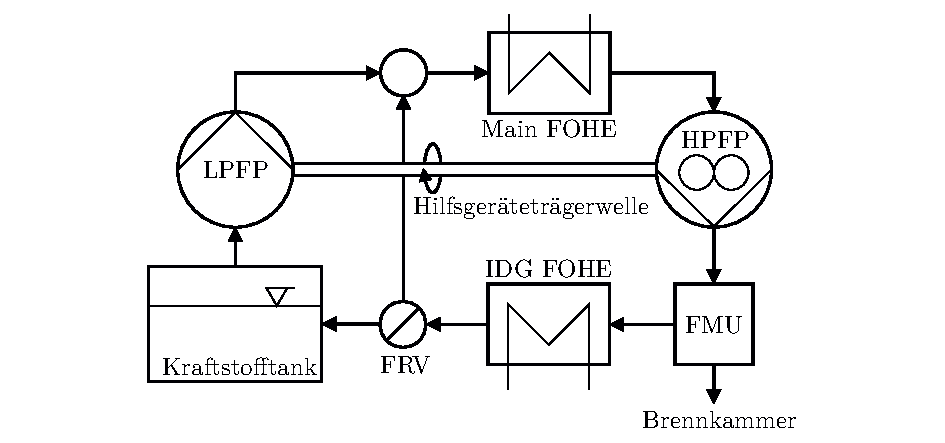
\includegraphics[width=1\linewidth]{4_Abbildungen/2_Hauptteil/Kraftstoffsystem Abbildungen/CFM56 Kraftstoffsystem 2.pdf}
  \caption{Kraftstoffsystems des CFM56-5B Triebwerks nach \cite{LinkeDiesinger.2014}}
  \label{fig:2.1}
\end{figure}
\FloatBarrier

Die in den Kraftstofftanks integrierten Boosterpumpen (in Abbildung \ref{fig:2.1} nicht abgebildet) versorgen die Triebwerke mit Kraftstoff. Im CFM56-5B Triebwerk wird der Kraftstoff zunächst von der Niederdruckpumpe in das Niederdrucksystem gefördert. Anschließend erfolgt eine Mischung mit warmem, rezirkuliertem Kraftstoff aus dem Hochdrucksystem. Nachdem der Kraftstoff in einem Wärmeübertrager für das Hauptölsystem weiter erwärmt wurde, durchläuft er den Kraftstofffilter und die Hochdruckpumpe.

Der Filter des CFM56-5B Triebwerks ist branchenüblich mit einem von einem Druckdifferenzsensor gesteuerten Bypass-Ventil ausgestattet, das im Falle einer Verstopfung aktiviert wird. Der Kraftstoffmassenstrom und -druck in die Brennkammer werden durch die Kraftstoffregeleinheit gesteuert, die im CFM56-5B Triebwerk auch als hydromechanische Einheit (engl.: Hydromechanical Unit, HMU) bezeichnet wird. Überschüssiger Kraftstoff durchläuft zunächst den Wärmeübertrager des Stromgenerator-Ölsystems und erreicht anschließend das Kraftstoff-Rückführventil (engl.: Fuel Return Valve, FRV). Je nach Öltemperatur bestimmt das Wärmemanagementsystem des CFM56-5B Triebwerks anhand eines Kennfeldes, welcher Kraftstoffmassenstrom in die Kraftstofftanks zurückgeleitet wird. Der restliche Kraftstoff wird in das Niederdrucksystem zurückgeführt. Die Kraftstofftemperatur wird vom Wärmemanagementsystem des CFM56-5B Triebwerk nicht berücksichtigt. \cite{Braunling.2015, LinkeDiesinger.2014}

\section{Wasserstoff-Kraftstoffsysteme}

Die Kraftstoffsysteme wasserstoffbetriebener Triebwerke müssen viele der gleichen Funktionen wie Kerosin-Kraftstoffsysteme erfüllen. Aufgrund der abweichenden Kraftstoffeigenschaften ergeben sich jedoch spezifische Herausforderungen. Da der Wasserstoff für Luftfahrtanwendungen in flüssiger, also kryogener Form bei niedrigen Temperaturen gespeichert wird, stellt die Vorkonditionierung eine besondere Herausforderung dar. Die Kombination aus niedrigeren Lagertemperaturen und der hohen spezifischen Wärmekapazität von Wasserstoff führt zu einem hohen Energiebedarf. \cite{Rompokos.2024, Sethi.2022}

Aus diesem Grund werden in der Literatur neben den aus konventionellen Kraftstoffsystemen bekannten Wärmeübertragern mit den Ölsystemen auch Wärmeübertrager innerhalb des thermodynamischen Kreisprozesses des Triebwerks untersucht (siehe Abbildung \ref{fig:2.2}). Diese sogenannten fortschrittlichen Kreisprozesse könnten nicht nur zusätzliche Wärmeeinträge in das Kraftstoffsystem liefern, sondern auch den Gesamtwirkungsgrad des Triebwerks steigern \cite{Tacconi.2023}.

\begin{figure}[ht]
\centering
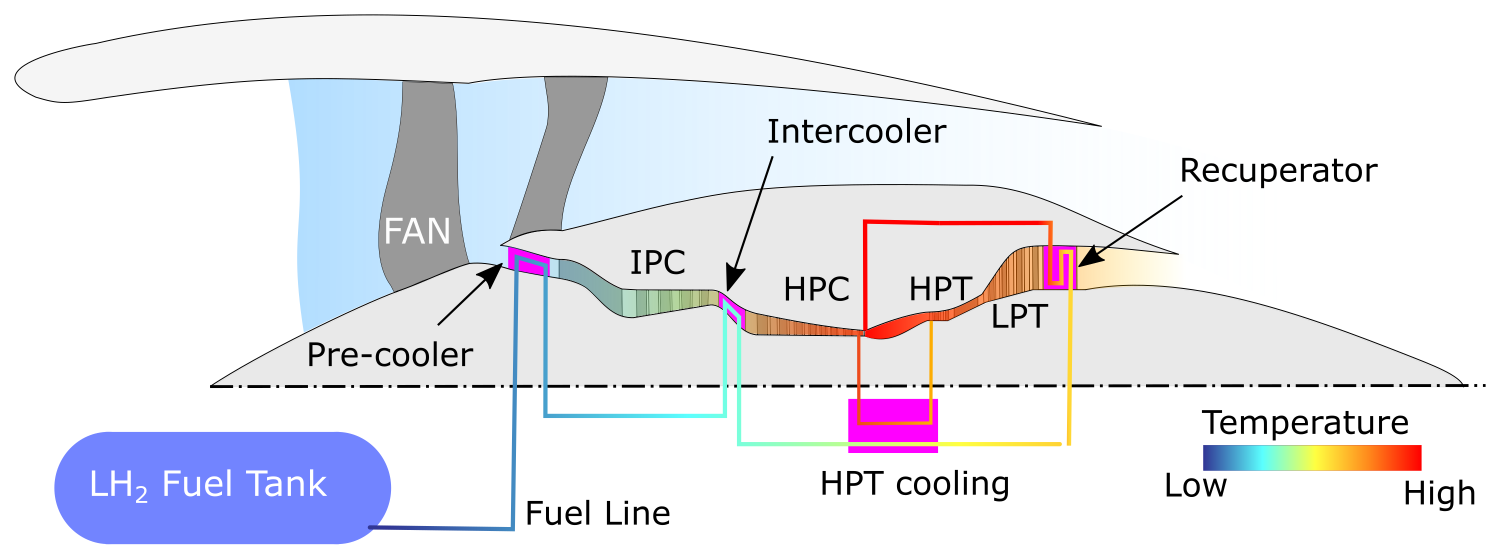
\includegraphics[width=0.75\linewidth]{4_Abbildungen/2_Hauptteil/Advanced Cycles.png}
  \caption{Wärmeübertrager fortschrittlicher Kreisprozesse \cite{Sethi.2022}}
  \label{fig:2.2}
\end{figure}
\FloatBarrier 

Zu den untersuchten fortschrittlichen Kreisprozessen zählen Vor-/Zwischenkühler, die durch geringere Eintrittstemperaturen der Luft in die Verdichter des Kerntriebwerks deren Arbeitsbedarf reduzieren \cite{Abedi.2022}. Wärmerückgewinnungssysteme im Abgas der Niederdruckturbine, sogenannte Rekuperatoren, senken die Abgastemperatur und erhöhen dadurch den Gesamtwirkungsgrad des Kreisprozesses \cite{Brewer.1991}. Eine Vorkühlung der Turbinenkühlluft in einem eigenen Wärmeübertrager könnte den benötigten Massenstrom an Kühlluft verringern und so den Turbinenwirkungsgrad steigern \cite{Brewer.1991}. Die Integration dieser Wärmeübertrager in den Kreisprozess des Triebwerks ist jedoch mit erheblichen finanziellen und technischen Risiken verbunden, weshalb ein Einsatz in der ersten Generation wasserstoffbetriebener Flugzeugtriebwerke als unwahrscheinlich gilt \cite{Rompokos.2024, Huete.2021}. 

Da sich diese Arbeit primär mit der Nachrüstung von kerosinbetriebenen Flugtriebwerken für die Nutzung mit Wasserstoff befasst, werden fortschrittliche Kreisprozesse nicht näher betrachtet. Das Wärmemanagement von Wasserstoff-Kraftstoffsystemen hält die Temperaturen der Ölsysteme innerhalb ihrer Betriebsgrenzen und stellt eine Mindesttemperatur des Kraftstoffs sicher. Im Folgenden werden mögliche Komponenten von Wasserstoff-Kraftstoffsystemen diskutiert und eine Kraftstoffsystemarchitektur aus der Literatur beschrieben.

\subsection{Kraftstoffpumpen}

Die Druckerhöhung des Kraftstoffs erfolgt bei den in der Literatur vorgeschlagenen Wasserstoff-Kraftstoffsystemen in zwei Schritten \cite{Ebrahimi.2024}. Für die Niederdruckpumpe wird eine redundante Ausführung in Form von mehreren im Kraftstofftank versenkten Kreiselpumpen vorgeschlagen. Die Niederdruckpumpen des Wasserstoff-Kraftstoffsystems übernehmen die Funktion der Boosterpumpen und der Niederdruckpumpe des Kerosin-Kraftstoffsystems. Aufgrund der physischen Distanz zu den Triebwerkswellen werden diese Pumpen elektrisch angetrieben \cite{Scholz.2003}. 

Für die finale Druckerhöhung gibt es in der Literatur unterschiedliche Ansätze. Das Pumpen von Wasserstoff im flüssigen Zustand erfordert vergleichsweise wenig Energie, jedoch sind Pumpen für kryogenen Wasserstoff aufgrund der unzureichenden Schmierwirkung des Kraftstoffs störanfällig. Bacic et al. \cite{BacicMarkoCoullJohn.2024} schlagen daher vor, den Kraftstoff nach erfolgter Verdampfung zu verdichten, um längere Wartungsintervalle zu ermöglichen. Für die Hochdruckpumpe beziehungsweise den Hochdruckverdichter ist sowohl ein Antrieb über die Hochdruckwelle als auch ein elektrischer Antrieb denkbar. Aufgrund der erforderlichen Druckverhältnisse bei hohem Schubbedarf, erfordert die Verdichtung im gasförmigen Zustand mehrere Verdichterstufen. Für die Druckerhöhung im flüssigen Zustand werden sowohl Kreiselpumpen als auch Verdrängerpumpen diskutiert \cite{Scholz.2003, Shaffer.2014}.

\subsection{Wärmeübertrager}

Neben den aus den Kerosin-Kraftstoffsystemen bekannten Wärmeübertragern mit den Ölsystemen bietet sich aufgrund des niedrigen Temperaturniveaus des flüssigen Wasserstoffs die Integration eines Wärmeübertragers mit dem Kabinen-Klimasystem (engl.: Environmental Control System, ECS) an \cite{Brewer.1991}. Das ECS wird mit Verdichter-Zapfluft versorgt, die vor ihrer Nutzung in der Kabine zunächst abgekühlt wird. In konventionellen Triebwerken wird hierfür ein mit Fan-Zapfluft gekühlter Wärmeübertrager eingesetzt. Durch einen Wärmeübertrager zwischen Wasserstoff und ECS kann der Fan-Zapfluftbedarf reduziert und zusätzliche Wärme für das Wasserstoff-Kraftstoffsystem gewonnen werden. 

Patrao et al. \cite{Patrao.2024} diskutieren die Problematik der Eisbildung in kryogenen Wärmeübertragern im Wasserstoff-Kraftstoffsystem. Ein möglicher Lösungsansatz ist die Rezirkulation des Wasserstoffs innerhalb des Kraftstoffsystems. Hierbei wird warmer Wasserstoff aus dem Hochdrucksystem vor den Eintritt in die betroffenen Wärmeübertrager rezirkuliert, um die Eintrittstemperatur des Wasserstoffs in die Wärmeübertrager so weit zu erhöhen, dass die luftseitigen Temperaturen des Wärmeübertragers stets oberhalb des Gefrierpunkts von Wasser bleiben \cite{Brewer.1991}. 

\subsection{Wärmemanagementsystem}

Das Wärmemanagementsystem von Wasserstoff-Kraftstoffsysteme unterscheidet sich in zwei Kernpunkten von konventionellen Kraftstoffsystemen. Zum einen ist es in der Regel nicht möglich, einen signifikanten Kraftstoffmassenstrom in die Kraftstofftanks rückzuführen, da der rückgeführte Wasserstoff wieder verflüssigt werden müsste. Eine Rückführung des Wasserstoffs für Zwecke des Wärmemanagements ist allerdings auch nicht erforderlich. Im Gegensatz zu Kerosin-Kraftstoffsystemen ist der Kraftstofftemperatur bei den Wasserstoff-Kraftstoffsystemen keine technische Obergrenze gesetzt. Im Gegenteil: Um Vereisungsprobleme aufgrund niedriger Kraftstofftemperaturen in der Brennkammer zu vermeiden, könnte neben der verfügbaren Abwärme auch der Einsatz weiterer Wärmequellen erforderlich sein. Als Alternative zu den zuvor diskutierten fortschrittlichen Kreisprozessen schlagen Palmer et al. \cite{PalmerChloeJWhurrJohnR.2024} vor, die für die Vorkonditionierung benötigte Wärme durch eine mit Fan-Zapfluft versorgte parallele Wasserstoffverbrennung bereitzustellen. Des Weiteren diskutiert der CRYOPLANE-Bericht \cite{Scholz.2003} die Erwärmung des Wasserstoffs im transienten Betrieb mit einer elektrischen Widerstandsheizung.

\subsection{Anordnung der Kraftstoffsystemkomponenten}

Brewer \cite{Brewer.1991} beschreibt in seinem Buch einen denkbaren Ansatz für Wasserstoff-Kraftstoffsysteme. Abbildung \ref{fig:brewer} enthält einen schematische Darstellung der Anordnung der Kraftstoffsystemkomponenten des Kraftstoffsystems von Brewer.


\begin{figure}[ht]
\centering
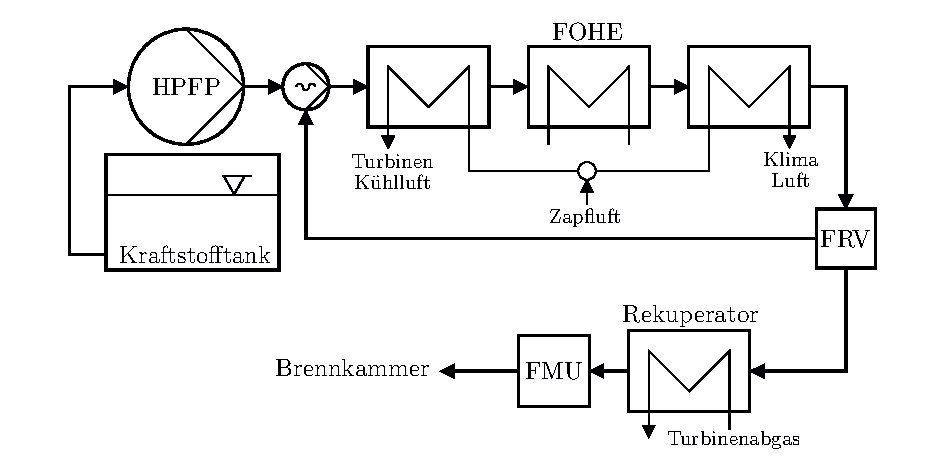
\includegraphics[width=1\linewidth]{4_Abbildungen/2_Hauptteil/Kraftstoffsystem Abbildungen/brewer.pdf}
  \caption{Wasserstoff-Kraftstoffsystem frei nach Brewer \cite{Brewer.1991}}
  \label{fig:brewer}
\end{figure}
\FloatBarrier 

Der flüssige Wasserstoff wird unter Überdruck in einem in die Zelle des Flugzeugs integrierten Kraftstofftank  gelagert. Eine elektrisch angetriebenen Kreiselpumpe fördert den Kraftstoff aus dem Tank in das Triebwerk. Im Triebwerk wird der flüssige Wasserstoff von der Hochdruckpumpe über den Brennkammerdruck gefördert. Im Anschluss an die Hochdruckpumpe, die ebenfalls als Kreiselpumpe ausgeführt ist, wird der geförderte Wasserstoff in einer Strahlpumpe als Treibmedium verwendet, um den rezirkulierten gasförmigen Wasserstoff zu fördern. Der rezirkulierte Wasserstoff gibt Wärme an den flüssigen Wasserstoff ab, wodurch dieser verdampft und auf eine Temperatur von \SI{200}{K} erwärmt wird. 

Der gemischte Wasserstoffstrom durchläuft wird anschließend in einer Reihe von Wärmeübertragern durch die Turbinenkühlluft, das Hauptölsystem und die Klimaluft erwärmt. Hinter den Wärmeübertragern wird der rezirkulierte Massenstrom in einem Kraftstoff-Rückführventil abgezapft. Der verbleibende Kraftstoff durchläuft anschließend einen Rekuperator, der den Wasserstoff auf eine Temperatur von \SI{677}{K} erhitzt. Abschließend wird der Wasserstoff durch die Kraftstoffregeleinheit in die Brennkammer geleitet.